In this section we discuss the algorithms evaluated in our two online
trials\footnote{All code used in these experiments is available at
\url{http://code.google.com/p/social-recommendation/}.  The conditions
of our ethics approval \#2011/142 from the Australian National
University for conducting human trials on Facebook require our
privacy policy
(\url{http://dmm.anu.edu.au/linkr/website/pp.php}) to
prohibit public sharing of data collected during these experiments.}
and additional analysis regarding trends and patterns in our social
recommendation setting.

\subsection{First Trial}

In our first trial, our objective was to evaluate four CF and SCF
approaches to establish which was the most promising direction for
SCF extension:
\begin{enumerate}
\item {\bf $k$-Nearest Neighbor (KNN)}: See Section~\ref{sec:nn}.
\item {\bf Support Vector Machines (SVM)}: See Section~\ref{sec:cbf}.
\item {\bf Matchbox (Mbox)}: Optimization of the $L_2$ regularized
Matchbox objective:
$$\Obj_\pmcf + \lambda \Obj_\ru + \lambda \Obj_\rv$$
\item {\bf Social Matchbox (Soc. Mbox)}: Optimization of the 
$L_2$ and \emph{feature socially regularized} Matchbox objective:
$$\Obj_\pmcf + \lambda_\rs \Obj_\rs + \lambda \Obj_\ru + \lambda \Obj_\rv$$
\end{enumerate}
Mbox and Soc. Mbox are optimized via gradient descent as outlined
in Appendix~\ref{app:Derivatives}.  All $\lambda$ parameters were manually
tuned in offline experiments.
KNN and MBox may be viewed as pure CF methods.  As discussed previously,
both SVM and Soc. Mbox may be viewed as SCF methods.  

The first live user trial was run from August 25 to October 13
with 108 users and yielded 2,493 like/dislike ratings of recommended
links over the 49 day period.  Algorithms were assigned randomly to the
users with counts shown in Table~\ref{tab:Assigned1} (left).

%%%%%%%%%%%%%%%%%%%%%%%%%%%%%%%%%%%%%%%%%%%%%%%%%%%%%%%%%%
\begin{table}[t!]
\centering
\begin{minipage}{1.5in}
\begin{tabular}{| l | c |}
\hline
{\bf Algorithm} & {\bf Users} \\
\hline
Soc. Mbox & 26\\
Mbox  & 26 \\
SVM & 28 \\
KNN & 28 \\
\hline
\end{tabular}
  \end{minipage}
  \begin{minipage}{1.3in}
\begin{tabular}{| l | c |}
\hline
{\bf Algorithm} & {\bf Users} \\
\hline
Soc. Mbox & 26\\
Spec. Mbox  & 25 \\
Spec. CP & 27 \\
Soc. Hybrid & 25 \\
\hline
\end{tabular}
  \end{minipage}
\caption{Number of users assigned per algorithm in the first trial (left)
and second trial (right).}
\label{tab:Assigned1}
\end{table}
%%%%%%%%%%%%%%%%%%%%%%%%%%%%%%%%%%%%%%%%%%%%%%%%%%%%%%%%%%

As shown in Figure~\ref{fig:OnlineResult1}, Social Matchbox was the
best performing algorithm in the first trial and in fact was the only
algorithm to receive more like ratings than dislike ratings. This
would suggest that using social information in conjunction with
MF-based CF does indeed provide useful information.  We also note a
significant drop in performance between recommending friend links and
recommending non-friend links, indicating that users had a bias to
like links recommended by friends more (importantly, we note that
users could see the friends who had already posted the link along with
their comments).

%%%%%%%%%%%%%%%%%%%%%%%%%%%%%%%%%%%%%%%%%%%%%%%%%%%%%%%%%%
\begin{figure*}[t!]
\centering
\subfigure{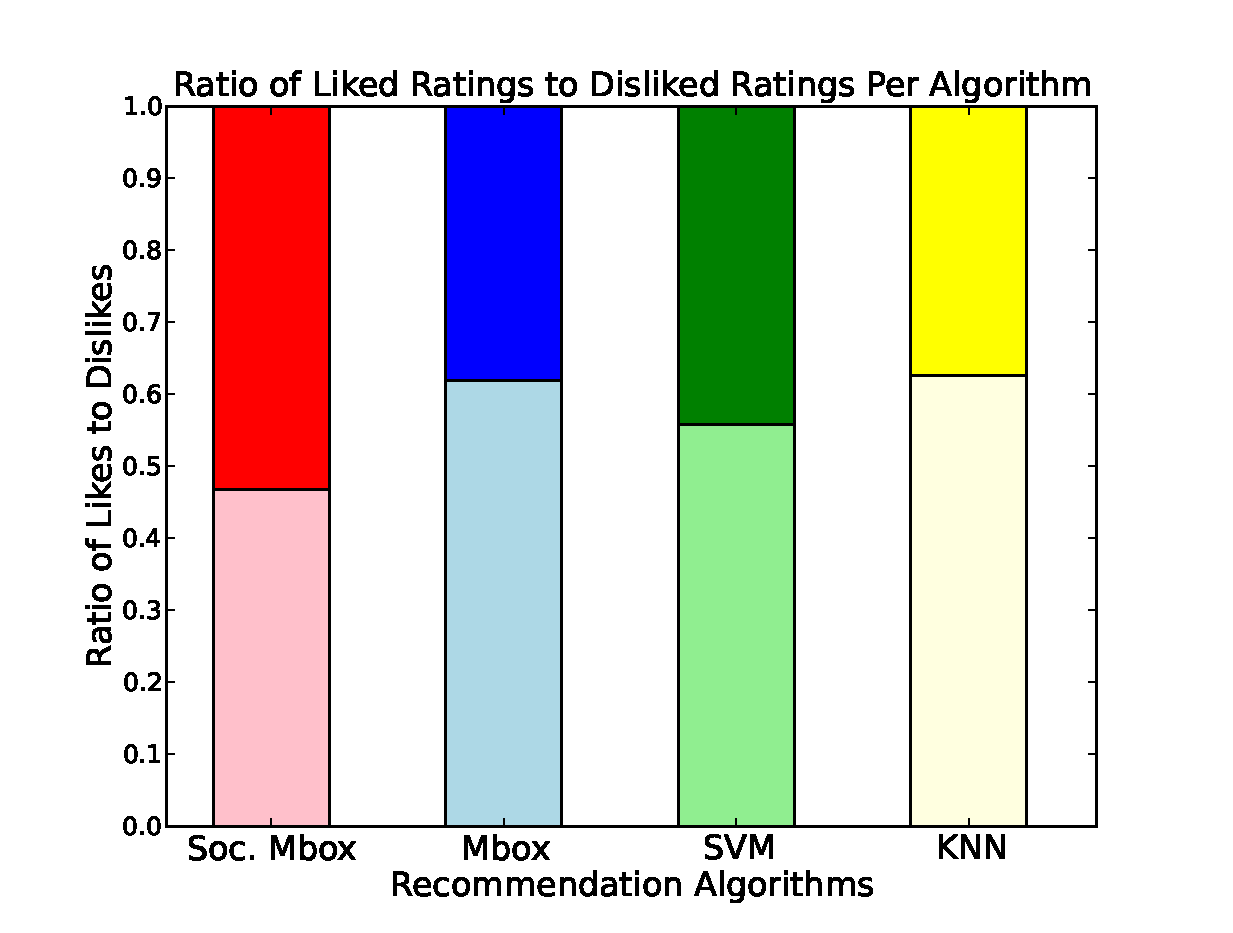
\includegraphics[scale=0.28]{img/live-likes1.eps}}
\subfigure{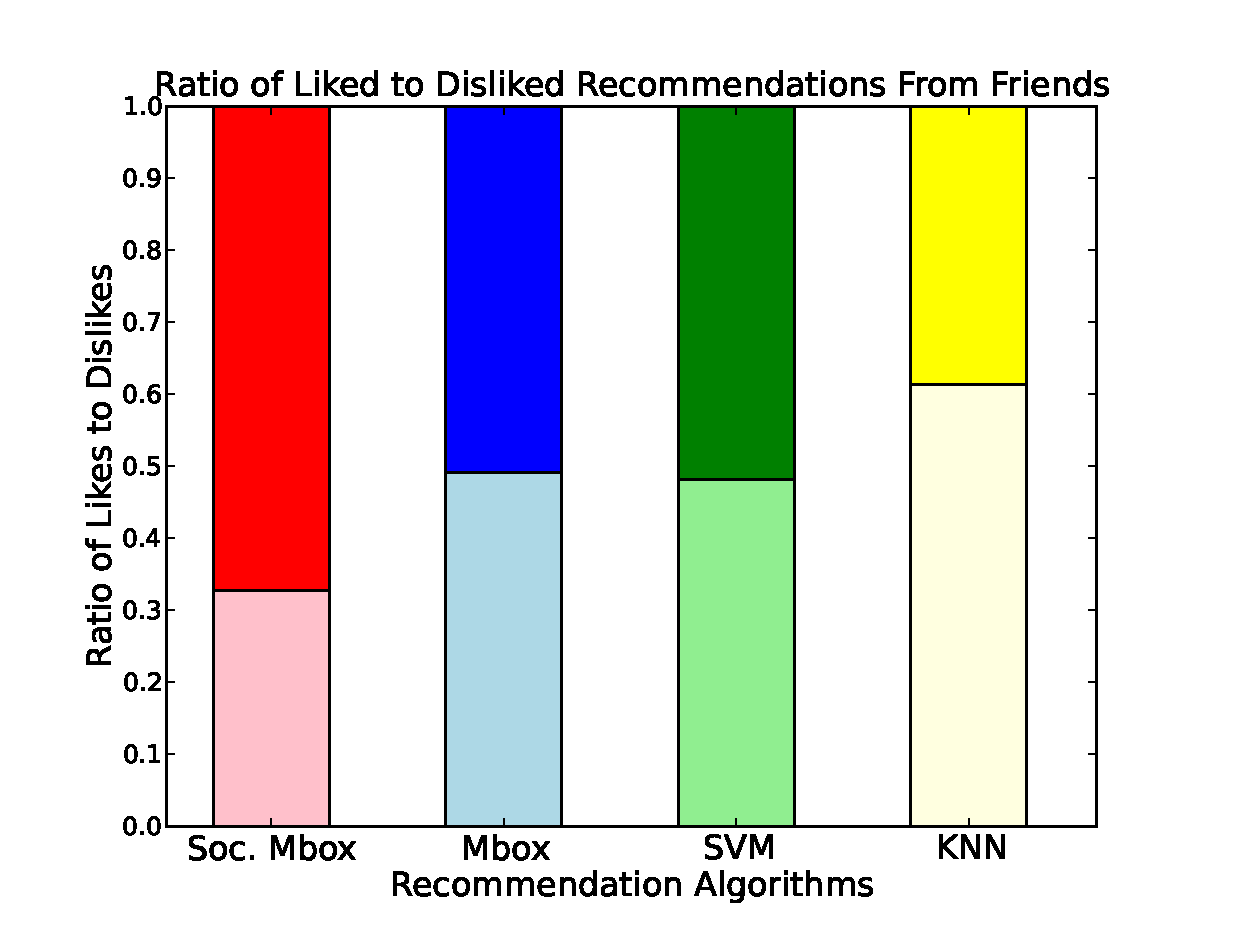
\includegraphics[scale=0.28]{img/live-friend-likes1.eps}}
\subfigure{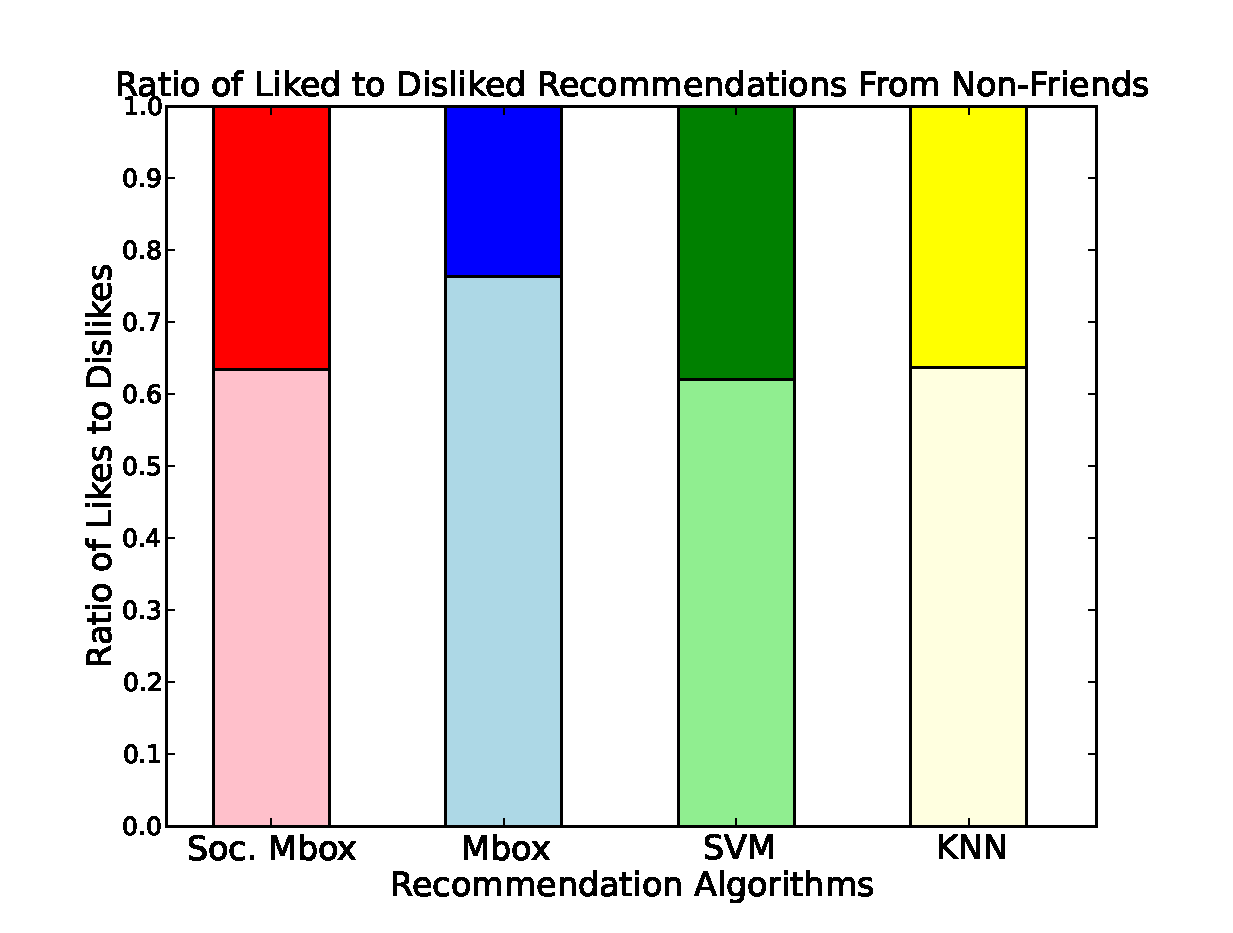
\includegraphics[scale=0.28]{img/live-nonfriend-likes1.eps}}
%\subfigure{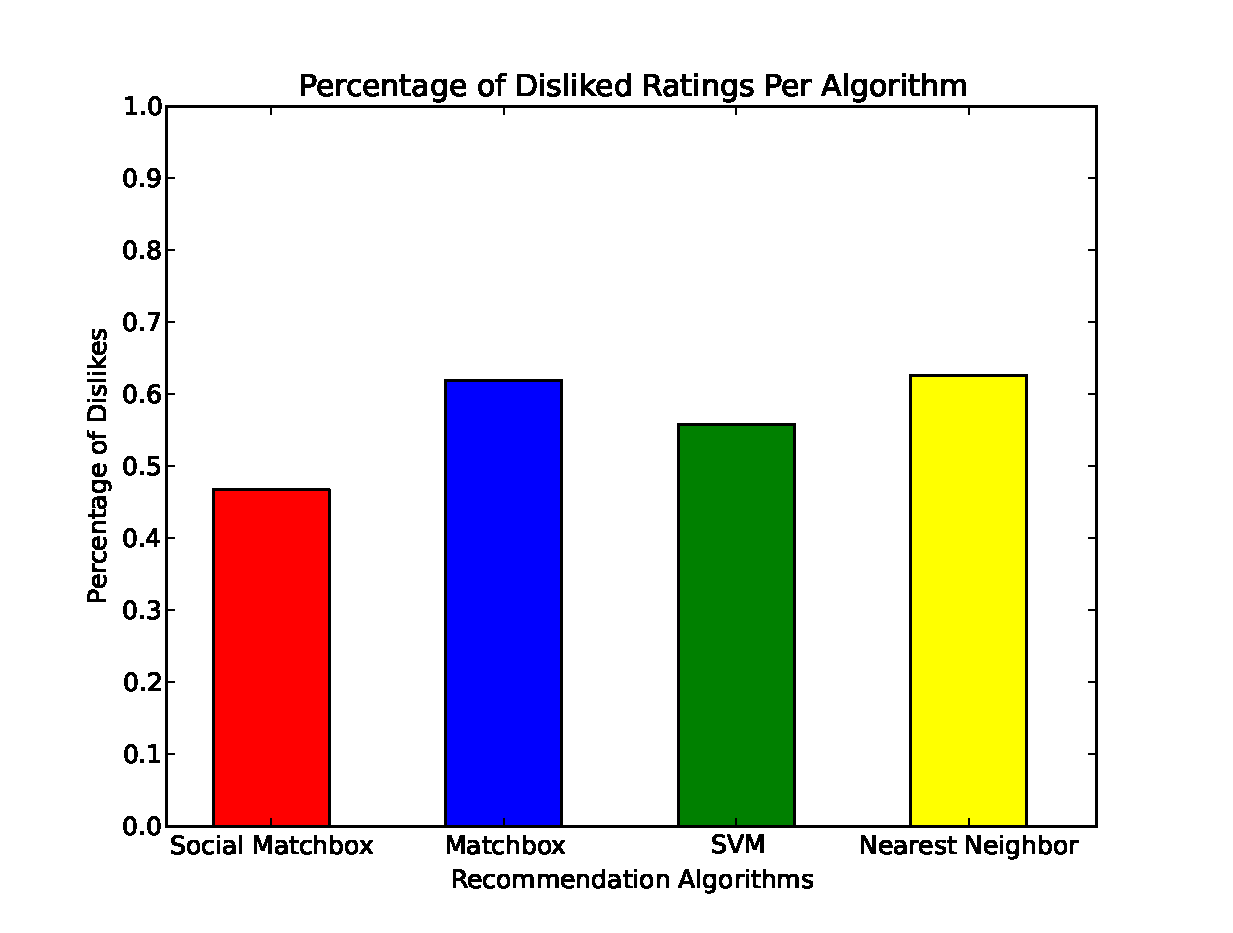
\includegraphics[scale=0.35]{img/live-dislikes1.eps}}
\caption{Stacked bar graphs of online results for the first 
user trial.  The fraction of likes is displayed above 
the fraction of dislikes.  (left) all links, (center) friend links,
(right) non-friend links.  The 95\% confidence interval on all 
results is $< \pm 0.02$ so all differences are signficant
except for MBox and SVM in the center and the virtual tie
between three algorithms on the right.}
\label{fig:OnlineResult1}
\end{figure*}
%%%%%%%%%%%%%%%%%%%%%%%%%%%%%%%%%%%%%%%%%%%%%%%%%%%%%%%%%%

%%%%%%%%%%%%%%%%%%%%%%%%%%%%%%%%%%%%%%%%%%%%%%%%%%%%%%%%%%
%%%%%%%%%%%%%%%%%%%%%%%%%%%%%%%%%%%%%%%%%%%%%%%%%%%%%%%%%%

\subsection{Second Trial}

For the second online trial, we again chose four algorithms to
randomly assign to the LinkR application users.  Social Matchbox
was included again as a baseline since it was the best performing
algorithm in the first trial.  The remaining three algorithms
were all orthogonal extensions (or variants) of Social Matchbox
based on the three novel objective functions defined in 
Section~\ref{sec:newobjfun_defs}:
\begin{itemize}
\item {\bf Social Matchbox (Soc. Mbox)} : unchanged.
\item {\bf Spectral Matchbox (Spec. Mbox)}: 
$$\Obj_\pmcf + \lambda_\rss \Obj_\rss + \lambda \Obj_\ru + \lambda \Obj_\rv$$
%Matchbox MF + Social Spectral Regularization + L2 $U$ Regularization + L2 $V$ Regularization
\item {\bf Social Hybrid (Soc. Hybrid)}: 
$$\Obj_\pmcf + \lambda_\rs \Obj_\rs + \lambda_\phy \Obj_\phy + \lambda \Obj_\ru + \lambda \Obj_\rv$$
%Hybrid + Social Regularization + L2 $U$ Regularization + L2 $V$ Regularization + L2 $\w$ Regularization
\item {\bf Spectral Co-preference (Spec. CP)}: 
$$\Obj_\pmcf + \lambda_\rscs \Obj_\rscs + \lambda \Obj_\ru + \lambda \Obj_\rv$$
%Matchbox MF + Social Co-preference Spectral Regularization + L2 $U$ Regularization + L2 $V$ Regularization
\end{itemize}
All objectives are optimized via gradient descent as outlined
in Appendix~\ref{app:Derivatives}.  
All $\lambda$ parameters were manually tuned in offline experiments.

The second trial with the above algorithms ran from October 13, 2011
to November 5, 2011 with 103 users and yielded 1,435 like/dislike
ratings of recommended links over the 24 day period; on the start of
the second trial, users were notified that they would be randomly
assigned to new algorithms and encouraged to re-engage with the LinkR
App if they had not been using it.  The distribution of the algorithms
to the users is shown in Table~\ref{tab:Assigned1} (right).

%%%%%%%%%%%%%%%%%%%%%%%%%%%%%%%%%%%%%%%%%%%%%%%%%%%%%%%%%%%%%%%%%%%%%%%%%
\begin{figure*}[t!]
\centering
\subfigure{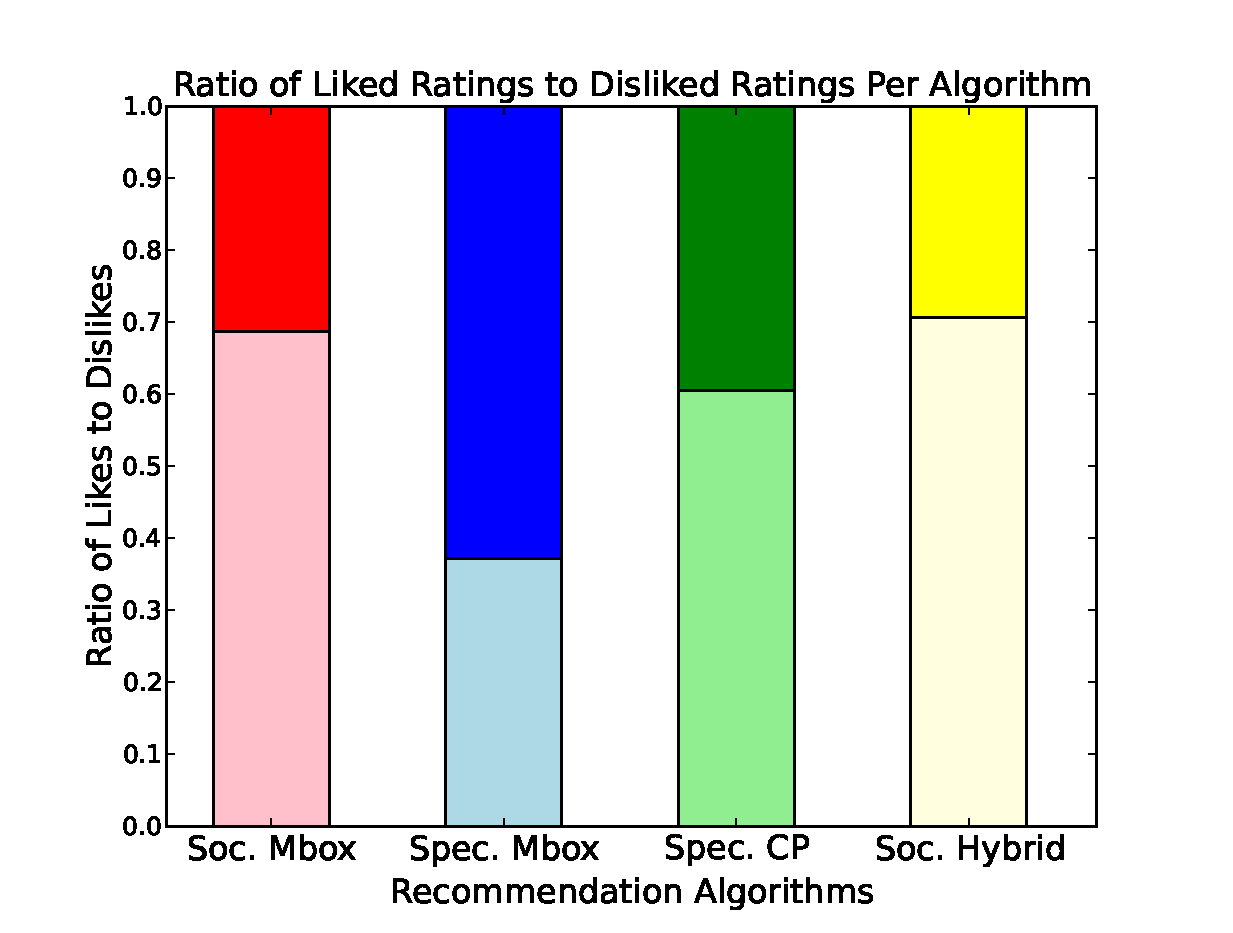
\includegraphics[scale=0.28]{img/live-likes2.eps}}
\subfigure{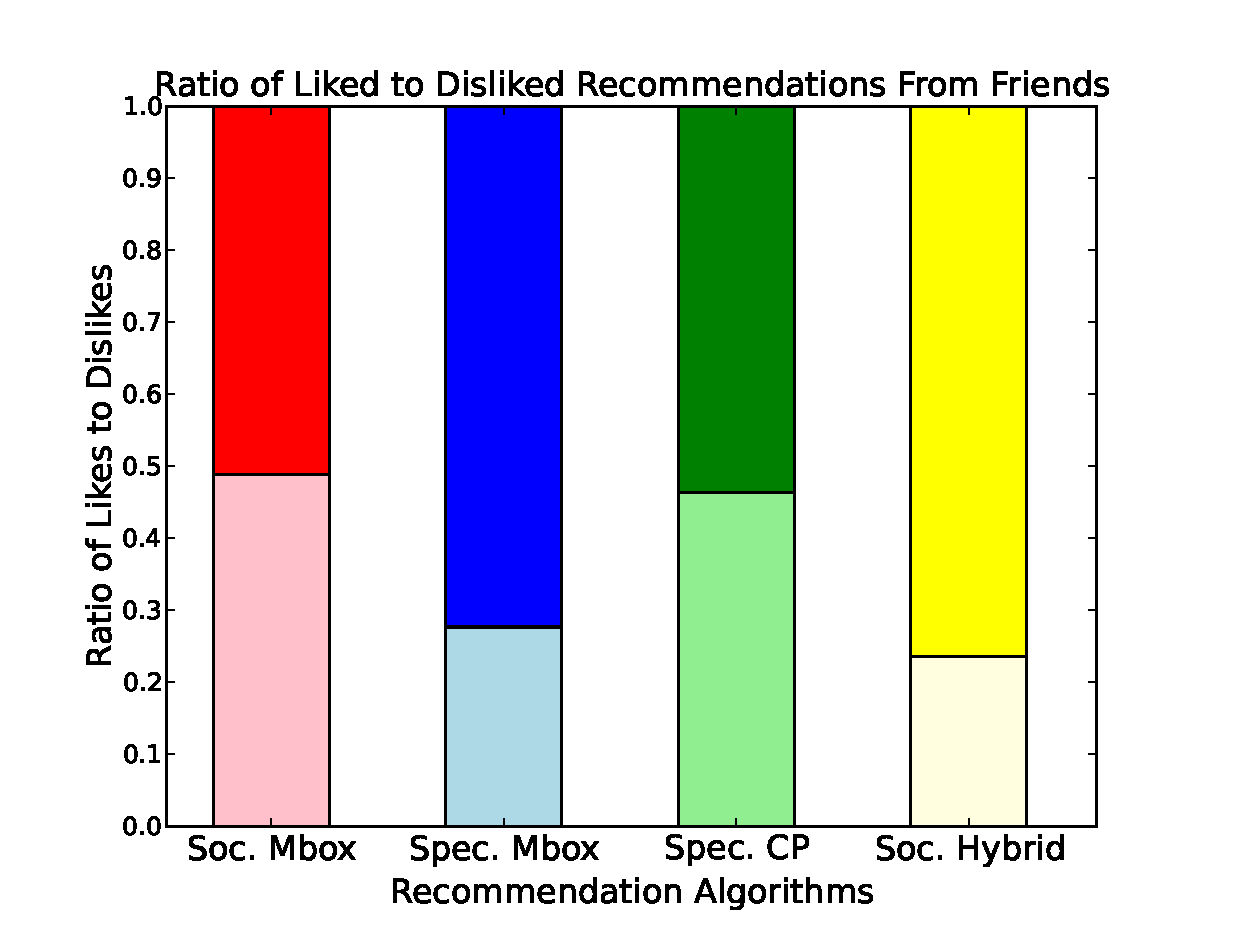
\includegraphics[scale=0.28]{img/live-friend-likes2.eps}}
\subfigure{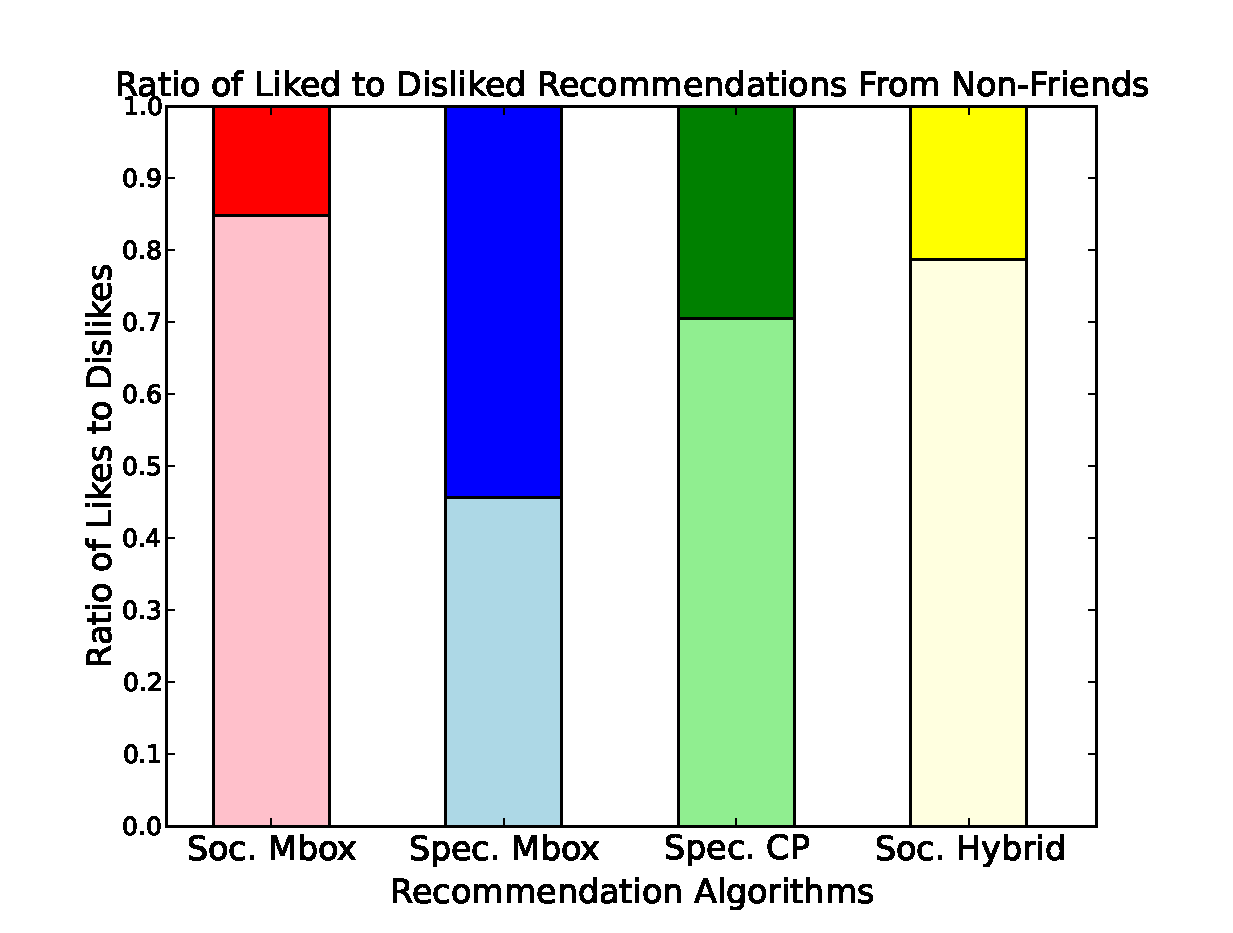
\includegraphics[scale=0.28]{img/live-nonfriend-likes2.eps}}
\caption{Stacked bar graphs of online results for the second
user trial.  The fraction of likes is displayed above 
the fraction of dislikes.  (left) all links, (center) friend links,
(right) non-friend links. The 95\% confidence interval on all 
results is $< \pm 0.026$ so all differences except Spec. Mbox
and Soc. Hybrid in the center graph are significant. }
\label{fig:online2}
\end{figure*}
%%%%%%%%%%%%%%%%%%%%%%%%%%%%%%%%%%%%%%%%%%%%%%%%%%%%%%%%%%%%%%%%%%%%%%%%%

{\bf TODO} 
Results shown in Figure~\ref{fig:online2}, observations:
\begin{itemize}
\item Spec. Mbox clearly the best and demonstrates that spectral social 
regularization is better than just social regularization.
\item Soc. Hybrid is capturing information diffusion well on friend links, 
nearly outperforming all other algorithms.
\item Spec. CP helps on non-friend links vs. baseline since it can capture 
information in copreferences of users even when they are not friends.
\end{itemize}

%%%%%%%%%%%%%%%%%%%%%%%%%%%%%%%%%%%%%%%%%%%%%%%%%%%%%%%%%%
%%%%%%%%%%%%%%%%%%%%%%%%%%%%%%%%%%%%%%%%%%%%%%%%%%%%%%%%%%

\subsection{Algorithm Independent Observations}

{\bf TODO: To save space we could merge both of the following
figures by dropping the center and right graphs of Figure~\ref{fig:click_evidence}
if we agree this is not too informative (interesting but not groundbreaking).
Otherwise we can keep as is.}

\subsubsection{Click evidence}

{\bf TODO:} Trying to show that clicks are not good
surrogates for like/dislike (warning to future experimenters!),
and that the reason for poor correlation isn't just lack of link context (seems
to have no impact) so people weren't just hating links with no context
that they clicked on to understand better, rather 
they hated links with/without context equally well.
Figure~\ref{fig:click_evidence}.

%%%%%%%%%%%%%%%%%%%%%%%%%%%%%%%%%%%%%%%%%%%%%%%%%%%%%%%%%%
\begin{figure*}[t!]
\centering
\subfigure{\includegraphics[scale=0.28]{img/clickedLikes.eps}}
\subfigure{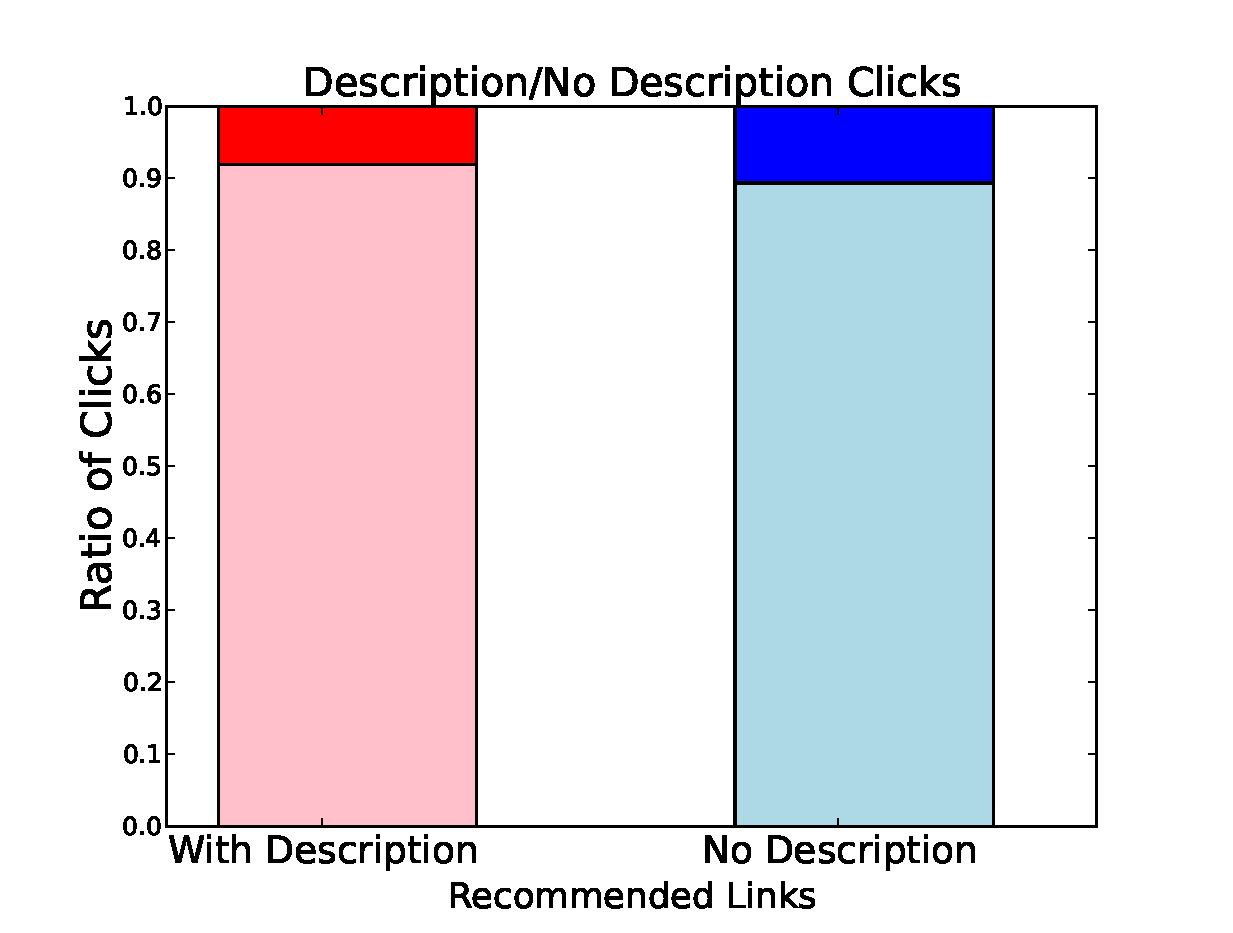
\includegraphics[scale=0.28]{img/descriptionClicked.eps}}
\subfigure{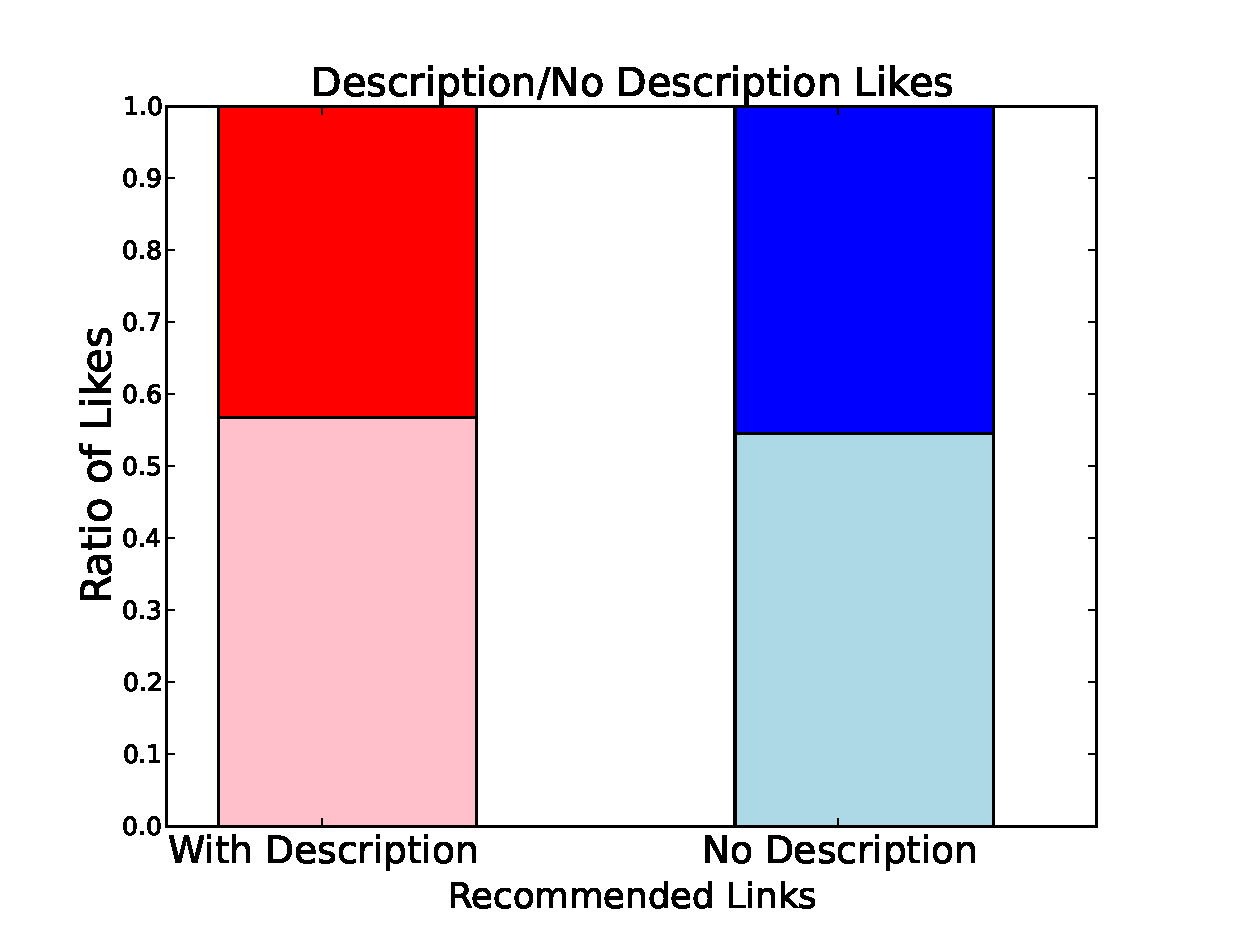
\includegraphics[scale=0.28]{img/descriptionLiked.eps}}
\caption{Stacked bar graphs of online results for the first 
user trial.  The fraction of likes (or clicks) is displayed above 
the fraction of dislikes (or non-clicks) and above fraction of not rated
links (if third bar segment present).  
(left) ratings for clicked links, (center) click rates if
text description not present, 
(right) percentage liked if click description not present.}
\label{fig:click_evidence}
\end{figure*}
%%%%%%%%%%%%%%%%%%%%%%%%%%%%%%%%%%%%%%%%%%%%%%%%%%%%%%%%%%

\subsubsection{Impact of Popularity}

{\bf TODO:} Links were sorted by global popularity (shares).
Users like esoteric (0-25\%) links as much, if not
more, than they like the most popular (75\%-100\%) (and again friends
more than non-friends but same general trend).  Most interesting
are the links that are kind of popular.
Figure~\ref{fig:popularity}.

%%%%%%%%%%%%%%%%%%%%%%%%%%%%%%%%%%%%%%%%%%%%%%%%%%%%%%%%%%
\begin{figure*}[t!]
\centering
\subfigure{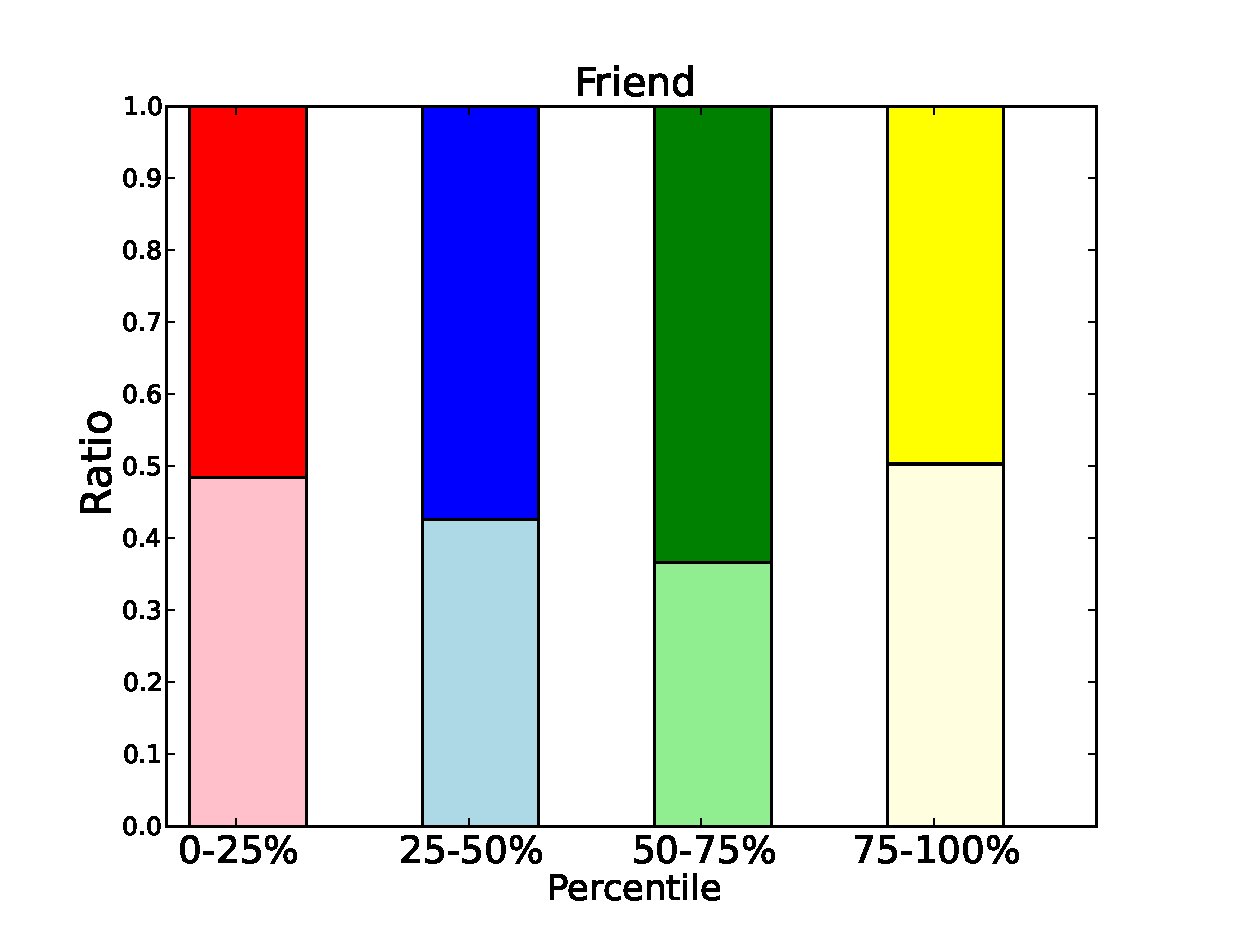
\includegraphics[scale=0.28]{img/percentileFriend.eps}}
\subfigure{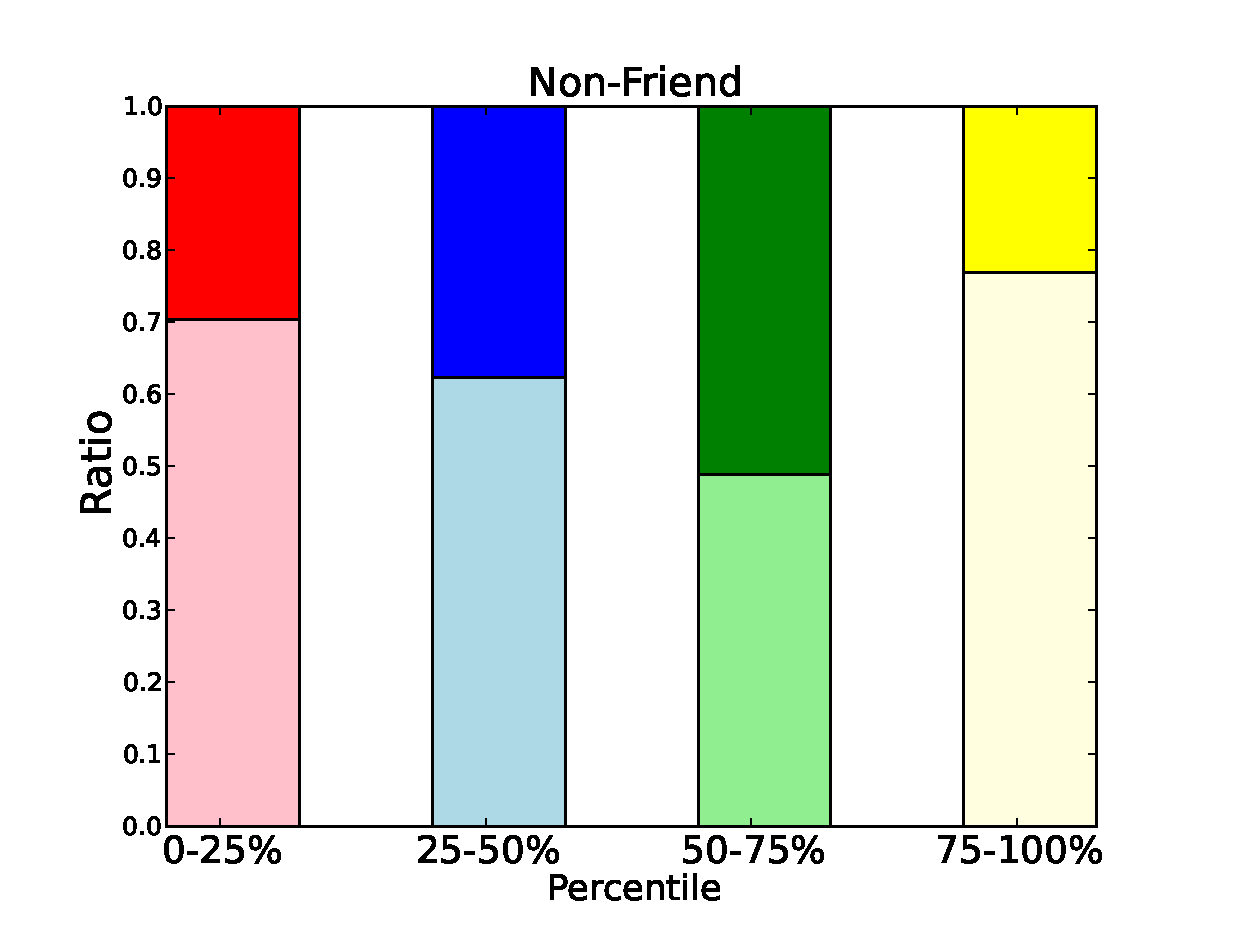
\includegraphics[scale=0.28]{img/percentileNon-Friend.eps}}
\caption{Stacked bar graphs of online results for the first 
user trial.  The fraction of likes is displayed above the fraction of
dislikes.  Shown are the ratings vs. quartile of popularity for (left)
friend and (right) non-friend links.}
\label{fig:popularity}
\end{figure*}
%%%%%%%%%%%%%%%%%%%%%%%%%%%%%%%%%%%%%%%%%%%%%%%%%%%%%%%%%%

